\documentclass[xelatex, 11pt, a4paper, ja=standard]{bxjsarticle}

% レポートの表紙のパッケージ
\usepackage{tuatreporttitle}
\usepackage{listings}
\usepackage{tikz}
\usepackage{caption}
\usepackage{graphicx} %スクショ
\usepackage{booktabs} % booktabsパッケージを追加
\usepackage{subfigure}
\usepackage{subfig}
\usepackage{fontspec}
\usepackage{xeCJK} % xeCJKパッケージを読み込む
\usepackage{url}
\usepackage{geometry}
\usepackage{lipsum}
\usepackage{amsmath} %式番号なくし
% \usepackage{texcount} %文字数カウント texcount filename.tex
\usepackage{placeins}


\usetikzlibrary{matrix}

%%%%%%%%%%%%%%%%%%%%
% ページの余白設定
%%%%%%%%%%%%%%%%%%%%
\geometry{reset, left=30mm, right=30mm, top=20mm, bottom=20mm}
%%%%%%%%%%%%%%%%%%%%

\usepackage{fancyhdr}


\pagestyle{fancy}
\fancyhf{}
\fancyfoot[C]{\thepage}
\renewcommand{\headrulewidth}{0pt}

%%%%%%%%%%%%%%%%%%%%
% 表紙設定
%%%%%%%%%%%%%%%%%%%%
% \title{実験報告書}	% タイトル(デフォルトで「実験報告書」)
\tuatgakunen{3}			% 学年
\tuatgakki{前期}		% 学期
\tuattani{2} 			% 単位
\tuatnumber{21266002} 	% 学籍番号
\tuattheme{RSA暗号} 		% テーマ
\tuatteacher{渡辺 先生} 		% 指導教員
\tuatkamoku{知能情報システム工学実験 2A} % 科目
\tuatauthor{赤坂 颯泰} 	% 氏名

% 共同作業者

% 作業日
\date1{2023年04月17日} 

% 提出期限
\duedate1{2023年04月30日}

% 提出日
\submitdate1{2023年04月30日}
%%%%%%%%%%%%%%%%%%%%


%%%%%%%%%%%%%%%%%%%%
% ここから実際のレポートの内容
%%%%%%%%%%%%%%%%%%%%
% e0ec9907


\begin{document}
% 表紙の作成
\maketitle
% ここから内容

\section{目的}
    代表的な公開鍵暗号であるRSA暗号について学び, 演習課題1~8を通してRSA暗号及び素数判定の実装を行うことを目的とする. 

\section{実験環境}
演習課題の実装にあたり, 言語はC++を用いた. \verb|#include <bits/stdc++.h> |
を行頭に記述することで, 標準ライブラリを全て読み込んだ. 
また, 一部C++17移行でサポートされている機能を使用したため, 
\verb|g++ <src-name>.cpp -std=gnu++17|
を実行することでコンパイルした. 
なお, 本実験で作成したプログラムは全て, 演習課題毎に付録として末尾に掲載した. 


\section{演習課題1 ユークリッドの互除法}
    ユークリッドの互除法とは, 2つの自然数a, bの最大公約数$gcd(a, b)$を時間計算量$O(log N)$で解くことができるアルゴリズムである. 

\subsection{演習課題1の目的}
    ユークリッドの互除法をプログラムで実装することを目的とした. 
    
\subsection{ユークリッドの互除法の設計}
自然数a, b(a>b)が与えられた時, $gcd(a, b) = gcd(b, a\%b)$が成り立つことを利用して, 
再帰関数を用いて実装した. 余りが0になった時点での余りを$a_i$とすると, $gcd(a, b)=a_i$を返り値として終了とした. 
なお, 入力のa, bについて, 素数と合成数の組み合わせをa>bという条件下で全通り試すために
\begin{itemize}
    \item $(\text{合成数, 合成数}) = (12, 8)$
    \item $(\text{素数, 合成数}) = (5, 4)$
    \item $(\text{合成数, 素数}) = (50, 5)$
    \item $(\text{素数, 素数}) = (41, 29)$
\end{itemize}
以上の四通りを採用した. 

\subsection{ユークリッドの互除法の実行結果}

\begin{figure}[htbp]
    \centering
    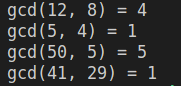
\includegraphics[height=0.15\textwidth,keepaspectratio]{./image/euclid.png}
    \caption{ユークリッドの互除法の出力結果}
    \label{fig:screenshot}
\end{figure}

図1より, 正しくユークリッドの互除法により, 入力値に対する最大公約数を出力できていることが確かめられた. 

\section{演習課題2 拡張ユークリッド}
    拡張ユークリッドとは, $gcd(a,b) = \alpha a+\beta b$を満たす整数の組$(\alpha, \beta)$を求めるアルゴリズムである. 
\subsection{演習課題2の目的}
拡張ユークリッドアルゴリズムを用い, 乗法逆元を求めるプログラムの作成を目的とする. 

\subsection{プログラムの設計}
引数に2つの整数a, b(a>b)を与えた, 法をNとした時, $ ay \equiv 1 \pmod {N} $となる乗法逆元yを求める関数modinvを作成した. 
$modinv$関数では, さらに内部で拡張ユークリッドアルゴリズムを計算するcalcExtendedEuclid関数を実装した. 
calcExtendedEuclid関数は, 引数に整数a, m, x, yをとった. 
それぞれax+by=1を満たす整数であり, gcd(a, b)を返り値としながら, ax+by=1を満たすx, yを計算した. 
これらの処理について, 演習課題1のcalcEuclid関数と同様に再帰的に計算を行った. 
calcExtendedEuclid関数で計算されたxに対して, mで割ったときの余りを正で返すmod関数を実装した. 
この余りをmodinv関数の返り値とした. 
なお, 入力のa, bについて, 演習課題1と同様に
\begin{itemize}
    \item $(\text{合成数, 合成数}) = (12, 8)$
    \item $(\text{素数, 合成数}) = (5, 4)$
    \item $(\text{合成数, 素数}) = (50, 5)$
    \item $(\text{素数, 素数}) = (41, 29)$
\end{itemize}
以上の四通りを採用し, a, b, x, yおよび逆元を出力した. 

\subsection{拡張ユークリッドの実行結果}

\begin{figure}[htbp]
    \centering
    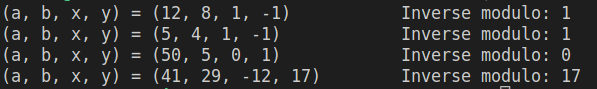
\includegraphics[height=0.15\textwidth,keepaspectratio]{./image/extendedEuclid.png}
    \caption{拡張ユークリッドの出力結果}
    \label{fig:screenshot}
\end{figure}

図2の結果について順にax+byを計算すると, 
12-8=4=gcd(12, 8), 5-4=1=gcd(5, 4), 
0+5=5=gcd(50, 5), 41×(-21)+29×17=1=gcd(41, 29)となった. 

また, bを法とした時の$a*x \equiv {1} \pmod{b}$を満たす整数xは, 
順に1, 1, 0, 17であった. 

\subsection{拡張ユークリッドの考察}
ax+byの計算結果が, 全て演習課1で求めた入力値に対する最大公約数に等しくなったことから, 
正しくユークリッドの拡張による演算が行われていることがわかった. 
一方で, 実行結果の逆元は1, 1, 0, 17であり, 理論的に$a*y \equiv {1} \pmod{b}$
を満たすyを順に求めると, 存在しない, 1, 存在しない, 17となる. 
このように結果が異なった理由は, 逆元が必ずしも存在する訳ではないためだと考える. 
実際に$a*y \equiv {1} \pmod{b}$を満たすyが存在するための必要十分条件は
$gcd(b, a)=1$であることが知られている. 
したがって, 理論的には逆元が存在し得ない組み合わせにおいて得られた実験結果は, 誤りだったといえる. 
よって, 乗法逆元を求めることができる入力値は, 互いに素な自然数の組み合わせに限ると考えられる. 

\section{演習課題3 RSA暗号による暗号化および復号化}
\subsection{演習課題3の目的}
素数p, qとeならびにメッセージ$m\in{1,....,N}$が与えられた時, RSA暗号による暗号化並びに復号化を行うプログラムの実装を目的とした. 

\subsection{プログラムの設計}
まず, 整数p, qについては標準入力で受け取った. nはpとqの積で求めた. 
eは, 第2節で実装したcalcEuclid関数の第一引数に(p-1)*(q-1), 第二引数にeを渡し, 
結果が1になるまで繰り返したときの試行回数をeとした. 
dは, 第2節で実装したmodinv関数の第一引数にe, 第二引数に(p-1)*(q-1)を渡した返り値とした. 
その後, RSA暗号による暗号化を行うencrptor関数を実装した. 
この関数は第一引数にe, 第二引数にnを渡した. 
この関数内では, 自然数mの初期値を0とし, mのe乗をnで割った余りを求める関数powerを計算した. 
この結果をcとすると, cが暗号化された値に相当する. 
mをインクリメントし, 繰り返し自乗法を使った法nのべき乗計算を行うpower関数によってn回暗号化を行った. 
暗号化の結果をangouという配列に格納した. 
次に, RSA暗号の復号化を行うdecriptor関数を作成した. 
この関数は, 第一引数にd, 第二引数にnをとった. 
さらに, angouの各要素を範囲for文を用いてcという変数名で順に取得し, power関数を用いてcのd乗をnで割った余りを計算することで復号化した. 
この復号化の結果をhirabunという配列に格納した. 
元のメッセージ$m\in{1,....,N}$と暗号化した配列angou, およびangouを復号化したhirabunを出力し, 
元のメッセージがhirabunと一致しているかどうかを判定した. 


\subsection{プログラムの実行結果及び考察}
RSA暗号による暗号化と復号化の結果を以下に示す. 

\begin{figure}[htbp]
    \centering
    \begin{center}
        \fbox{\parbox{0.9\textwidth}{
            $
            p: 13\\
            q: 7\\
            N: 91\\
            e: 5\\
            d: 29\\
            angou:  013261233141638818272381314717475448076212943351522784228852243442\\
            43461265666353618543773555685252679454849576789863697643940588762701511471\\
            61720777853199108328506068305990\\\\
            hirabun:012345678910111213141516171819202122232425262728293031323334353637\\
            38394041424344454647484950515253545556575859606162636465666768697071727374\\
            75767778798081828384858687888990\\
            $
        }
    }
\end{center}
\caption{RSA暗号による暗号化と復号化}
\label{fig:screenshot}
\end{figure}

hirabunは0~Nまでの値が順に並んだ数字列である. これを暗号化したところ図3のangouが得られた. 
さらに平文に復号化したところhirabunが得られた. 

\subsection{RSA暗号による暗号化と復号化の考察}
正しく\texttt{angou}が\texttt{hirabun}に変換されていることを確かめるために, \texttt{for}文で0からNまでの値を順にファイル出力し, \texttt{hirabun}と一致しているかを判定した. 
0からNまでの値を\texttt{hirabun\_1.txt}に, \texttt{hirabun}の内容を\texttt{hirabun\_2.txt}にファイル出力し, \texttt{diff -y}コマンドによって差分を出力した. その結果を以下に示す. 

\begin{figure}[htbp]
    \centering
    \begin{center}
        \fbox{\parbox{0.9\textwidth}{
            diff hirabun\_1.txt hirabun\_2.txt -y \\
            0123456789101112131415161718192021222324252627282930313233343   0123456789101112131415161718192021222324252627282930313233343
        }
    }
\end{center}
\caption{diff -yコマンドによる差分表示}
\label{fig:screenshot}
\end{figure}

図4より, 暗号化以前のhirabunに対して差分は見られなかった. 
よって, hirabunを正しく暗号化し, 復号化することができたと言える. 


\section{演習課題4 総当りによる素数判定法}
\subsection{演習課題4の目的}
総当たりによる素数判定法をプログラムで実装し, ビット長nを大きくしていったときの実行時間について調べることを目的とした. 

\subsection{プログラムの設計}
総当たりによる素数判定のアルゴリズムについて述べる. 
素数の候補をpとすると, pが$k=2, ... , \lfloor \sqrt{p} \rfloor$に対して順に割り切れるかどうかを調べた. 
すなわち, 
\begin{equation*}
    \forall k \in [2, \lfloor \sqrt{p} \rfloor], \quad p \not\equiv 0 \pmod{k} \Rightarrow isPrime
\end{equation*}
上式を実装した. 
ここでは$p=2,...,10^5$とし, そのうち素数と判定するまでの繰り返し回数を記録し出力した. 

\subsection{プログラムの実行結果}
総当りによる素数判定の結果を以下に示す. 
横軸を素数, 縦軸を反復回数の対数とした. 
\begin{figure}[htbp]
    \centering
    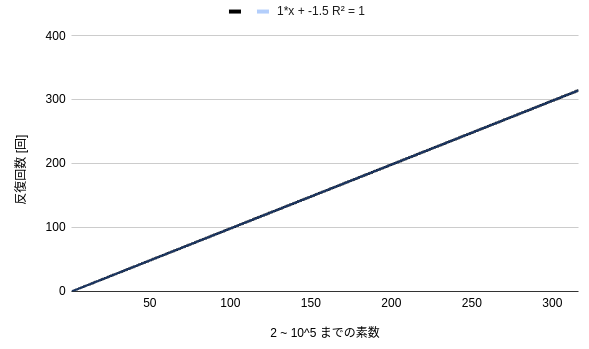
\includegraphics[height=0.5\textwidth,keepaspectratio]{./image/prime.png}
    \caption{素数の検出にかかる反復回数の出力結果}
    \label{fig:screenshot}
\end{figure}
\FloatBarrier %改ページに使えるやつ

上図の反復回数に対する片対数グラフの回帰直線は, 傾きは1であり素数の増大に伴い反復関数も比例する関係性が得られた. 
また, $R^2 = 1$であったことから, この関係性には非常に強い正の相関があると言える. 

\subsection{総当りにおける素数判定法の考察}
素数を判定する際には$sqrt(p)$回だけ試行するため, その時間計算量は$O(sqrt{p})$となると考えられる. 
そのために, 片対数を取った場合に図5のように比例した結果が得られたといえる. 
このように, 反復回数が素数の候補である数の長さに比例して指数的に増加してしまう. 
したがって, 総当りにおける素数判定法は, 効率的な素数判定法であるとはいえない. 


\section{演習課題5 フェルマーテスト}
フェルマーテストは, フェルマーの小定理を利用した乱択アルゴリズムに分類される素数判定法である. 
フェルマーの小定理とは, 
\begin{center}
    \fbox{\parbox{0.9\textwidth}{
        フェルマーの小定理:\\\
         $p>0$の素数に対して$1\leq a\leq p-1$とすると, 
        \begin{equation*}
            a^p \equiv a \pmod{p}
        \end{equation*}
    }}
\end{center}
上のような関係式が成り立つ定理である. 
この式を変形すると 
\begin{equation*} a^{p-1} \equiv 1 \pmod{p} \end{equation*}
となる. 
さらに対偶をとれば, 
\begin{equation*} a^{p-1} \not \equiv 1 \pmod{p} \end{equation*}
が成り立つならば, pは素数ではないと言える. 
また, 乱択アルゴリズム(Randomized Algorithm)とは, 乱数によって動作が決定されるアルゴリズムである. 
したがって, 必ずしも正しい判定が行われるとは限らない. 
一方で, 決定的な手続きに即したアルゴリズムと比較して高速に処理することが可能である. 
また, カーマイケル数とは, 合成数のうち
$a^{n-1} \equiv 1 \pmod{n}$
を満たす正の整数nのことである. 


\subsection{演習課題5の目的}
フェルマーテストをプログラムで実装し, カーマイケル数以外で誤判定確率を評価することを目的とした. 

\subsection{フェルマーテストの設計}
フェルマーテストのアルゴリズムについて述べる. 
\begin{center}
    \fbox{\parbox{0.9\textwidth}{
        フェルマーテスト:
        \begin{itemize}
            \item 入力: 素数の候補$p$, 最大繰り返し回数$S$ 
            \item 出力: $p$が素数である確率 [\%]
        \end{itemize}
        とし, $1 \leq i \leq S$の間以下の処理1$\sim$3を行った. 
        \begin{enumerate}
            \item $a \in \left\{1,2,...,p-1\right\}$ をランダムに選択した. 
            \item $a^{p-1} \not\equiv 1 \pmod{p} \Rightarrow \text{isNotPrime}$ 
            $\textrm{Otherwise} \Rightarrow \text{isPrime}$ として各回数を記録
            \item iをインクリメントし, ステップ1に戻る. 
        \end{enumerate}
    }}
\end{center}
なお, 乱数の生成にはC++標準ライブラリで提供される乱数生成器std::mt19937を用いた. 

\section{フェルマーテストの実験結果}
最も小さいカーマイケル数は561であるため, 561を含まない1~500までの数に対して素数になる確率を下図に示した. 
\begin{figure}[htbp]
    \centering
    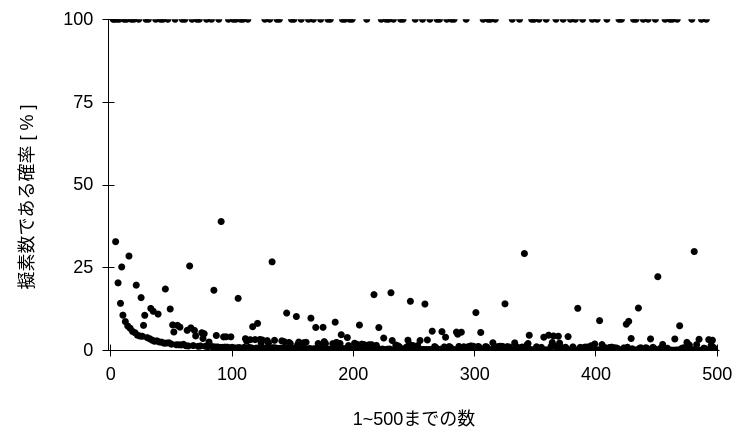
\includegraphics[height=0.5\textwidth,keepaspectratio]{./image/felmer.png}
    \caption{1~500に対するフェルマーテストの結果}
    \label{fig:screenshot}
\end{figure}

図5より, 素数は100\%の確率で素数だと判定され, 合成数の素数と判定される確率は全て50\%以下であった. 
合成数の素数判定確率が最も高かったものは91の38.98\%であった. 
したがって, カーマイケル数以外の合成数に対する素数判定は, 50\%を閾値とすると正常に機能しているといえる. 

\subsection{フェルマーテストの考察}
カーマイケル数におけるフェルマーテストの性能について考察する. 
カーマイケル数は小さい順に561, 1105, 1729, 2465, 2821, 6601, 8911であり, 
これらに対してフェルマーテストによって素数と判定される確率を調べた. 
その結果を下図に示す. 
\begin{figure}[htbp]
    \centering
    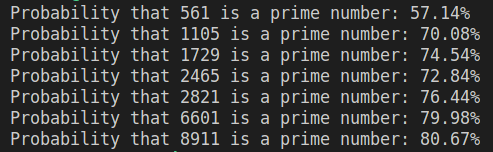
\includegraphics[height=0.15\textwidth,keepaspectratio]{./image/carmichael_felmer.png}
    \caption{カーマイケルに対するフェルマーテストの結果}
    \label{fig:screenshot}
\end{figure}
図7より, どのカーマイケル数に対しても50\%以上の確率で素数だと判定されていることがわかる. 
何故このような結果が得られたのかについて述べる. 
まず, フェルマーテストはフェルマーの小定理より, aとnを互いに素な自然数とすると, \begin{equation*} a^{p-1} \equiv 1 \pmod{p} \end{equation*}
を満たす場合, pを素数であると判定する. 
ここで, 全てのカーマイケル数は合成数でありながら, 上式を満たす互いに素な自然数$a$をもつ. 
したがって, フェルマーテストを通過すると考えられる. 
そのため, カーマイケル数に対して素数の誤判定を防ぐためには, 
フェルマーテストよりも条件が厳しい素数判定法を用いる必要があるといえる. 

\section{演習課題6 Miller-Rabinテスト}
演習課題5で実装したフェルマーテストではカーマイケル数に対しては正しく機能しない. 
この欠点を改善したアルゴリズムがMiller-Rabinテストである. 
このテストの根幹には次の性質がある. 
\begin{center}
    \fbox{\parbox{0.9\textwidth}{
        補題: $p$が素数であるとき, 自然数$a$が $a^{2} \equiv {1} \pmod{p}$を満たすならば, 
        $a \equiv \pm {1} \pmod{p}$が成り立つ. 

        補題の対偶: $a^{2} \equiv {1} \pmod{p} ∧$
        $a \not \equiv {\pm{1}} \pmod{p} $
        を満たす$a$が存在するならば, $p$は素数ではない. 
    }}
\end{center}
上記の補題の対偶を利用してMiller-Rabinを実装することが可能である. 

\subsection{演習課題6の目的}
Miller-Rabinテストをプログラムで実装し, カーマイケル数に対して誤判定確率を評価することを目的とした. 


\subsection{Miller-Rabinテストの設計}
Miller-Rabinテストのアルゴリズムについて述べる. 
\begin{center}
    \fbox{\parbox{0.9\textwidth}{
        Miller-Rabinテスト:
        \begin{itemize}
            \item 入力: 素数の候補$p$, 最大繰り返し回数$S$ 
            \item 出力: $p$が素数である確率 [\%]
        \end{itemize}
        とし, $1 \leq i \leq S$の間以下の処理1$\sim$3を行った. 
        \begin{enumerate}
            \item $a \in \left\{1,2,\ldots,p-1\right\}$ をランダムに選択. 
            \item if $a^{p-1} \not\equiv 1 \pmod{p} \Rightarrow \text{isNotPrime} \\
            \textrm{else if } j=1,\ldots,u$に対して, $a^{2^{j}v} \equiv {1} \pmod{p} 
            \land a^{2^jv} \not \equiv {\pm{1}} \pmod{p} $となる$j$が存在.$\Rightarrow \text{isNotPrime}$ \\
            $\textrm{Otherwise} \Rightarrow \text{isPrime}$ として各回数を記録
            \item i=Sならば終了. そうでなければ, iをインクリメントし, ステップ1に戻る. 
        \end{enumerate}
    }}
\end{center}
なお, 乱数の生成にはC++標準ライブラリで提供される乱数生成器std::mt19937を用いた. 
また本実験では$s=10^5$とした. 

\subsection{Miller-Rabinテストの実験結果}
フェルマーテストで扱ったカーマイケル数に対してMiller-Rabinテストを実行した場合の結果を以下に示す. 
\begin{figure}[htbp]
    \centering
    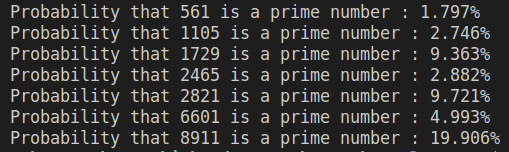
\includegraphics[height=0.15\textwidth,keepaspectratio]{./image/carmichael_miller-rabin.png}
    \caption{カーマイケル数に対するMiller-Rabinテストの結果}
    \label{fig:screenshot}
\end{figure}

フェルマーテストでは素数だと誤判定されていたカーマイケル数は, 素数と判定される確率が全て20\%以下となった. 
50\%を境界とすれば, 全てのカーマイケル数に対して正しく合成数と判定できているといえる. 

\subsection{Miller-Rabinテストの考察}
Miller-Rabinテストではカーマイケル数に対して有効である理由について述べる. 
カーマイケル数は, 前述の通りある自然数$n$を素因数分解したときに, $(n-1)$を因数に持ち, 
かつ全ての素因数$p$について$p-1$が$(n-1)$の約数であるような合成数である. 
この性質から, カーマイケル数$n$を素数と誤判定するためには, $n$のある素因数$p$に対して, 
Miller-Rabinテストによって$p$を素数と判定する必要がある. 
ところが, カーマイケル数にはこのような素因数$p$が複数存在する. 
よって, 全ての素因数がMiller-Rabinテストを通過する必要がある. 
しかし, その確率は非常に低いため, カーマイケル数に対してMiller-Rabinは有効であると考えられる. 

\section{演習課題7 素数生成}
\subsection{演習課題7の目的}
素数生成アルゴリズムに演習課題6で作成したMillar-Rabinテストを組み合わせ, 素数をランダムに生成するプログラムを実装することを目的とした. 

\subsection{素数生成器の設計}
本実験では素数をランダムに生成するアルゴリズムを採用した. 
以下にその具体的な処理について述べる. 

\begin{center}
    \fbox{\parbox{0.9\textwidth}{
        素数生成器:
        \begin{itemize}
            \item 入力: 生成したい素数の長さ$n$(ビット), 最大繰り返し回数$K$ 
            \item 出力: 素数か否かのbool値 初期値は$False$
        \end{itemize}
        とし, $1 \leq i \leq K$の間以下の処理1$\sim$3を行った. 
        \begin{enumerate}
            \item $(n-1)$ビットの整数$p'$を${\{0, 1\}}^{n-1}$ からランダムに選択. 
            \item 素数の候補を$p=1||p'$($p'$の先頭に1を付加した$n$ビットの整数)とした. 
            \item Miller-Rabinテストにより, $p$が素数であれば$True$を返し終了. そうでなければiをインクリメントし, ステップ1に戻る. 
        \end{enumerate}
    }}
\end{center}

本実験では, 入力したい素数の長さは16ビットとし, 最大繰り返し数を100回とした. 

\subsection{素数生成器の実験結果}
実験結果を下図に示す. 
\begin{figure}[htbp]
    \centering
    \begin{minipage}[b]{0.4\textwidth}
        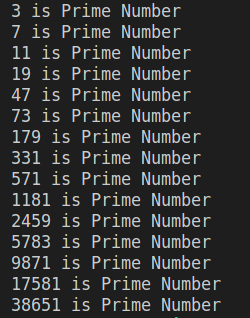
\includegraphics[width=\textwidth]{./image/primeGenerator_1.png}
        \label{fig:./image/primeGenerator_1.png}
    \end{minipage}
    \hfill
    \begin{minipage}[b]{0.4\textwidth}
        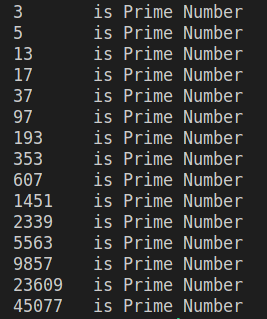
\includegraphics[width=\textwidth]{./image/primeGenerator_2.png}
        \label{fig:./image/primeGenerator_2.png}
    \end{minipage}
    \\
    \begin{minipage}[b]{0.4\textwidth}
        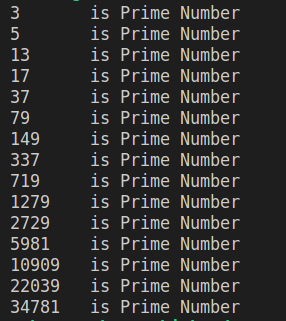
\includegraphics[width=\textwidth]{./image/primeGenerator_3.png}
        \label{fig:./image/primeGenerator_3.png}
    \end{minipage}
    \hfill
    \begin{minipage}[b]{0.4\textwidth}
        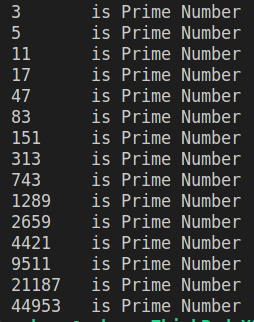
\includegraphics[width=\textwidth]{./image/primeGenerator_4.png}
        \label{fig:./image/primeGenerator_4.png}
    \end{minipage}
    \label{fig:素数生成器の実行結果}
    \caption{素数生成器の実行結果}
\end{figure}
\FloatBarrier %改ページに使えるやつ

素数生成器プログラムを4回実行した結果, n=15個の素数がそれぞれ生成された. 

\section{素数生成器の考察}
図9より, 素数のビット数が多くなるにつれて, 多様な素数を生成することが可能になると考えられる. 
例えばn=2の場合は2ビットで表せる素数は3のみである. よって, 4回の試行回数のどの結果でも2ビットの素数の出力結果は3で共通であった. 
ところが, n=16ビットで表せる素数は, $2^15から2^16-1$の数の範囲にある. 
故に, 図9で生成された数値は順に, 38651, 45077, 34781, 44953と全て異なる素数になったといえる. 
一般化すれば, $2^{n-1}から2^n-1$までの範囲にある数値からランダムに素数を生成することができる. 
したがって, 素数のビット数の増加に伴い, 生成可能な素数も増加するといえる. 


\section{演習課題8 RSA暗号システム}
\subsection{演習課題8の目的}
演習課題7の素数生成アルゴリズムと演習課題3の暗号化/復号化アルゴリズムを組み合わせ, RSA暗号システムを実装することを目的とした. 

\subsection{RSA暗号システムの設計}
RSA暗号システムを実現する関数calcRSASystemの実装について述べる. 
calcRSASystemには2つの素数を入力値として与える必要があるので, 
事前に演習課題7で作成したgeneratePrime関数を用いて素数$p, q$を求めた. 
ただし, $p, q$は互いに異なる素数である必要があるので, $q$が$p$と一致しないという条件を満たすまで, 
generatePrime関数を実行した. 
その後, $p, q$をcalcRSASystem関数に与えた. 
具体的なアルゴリズムについて以下に示す. 
\begin{center}
    \fbox{\parbox{0.9\textwidth}{
        calcRSASystem:
        \begin{itemize}
            \item 入力: 生成する素数のビット$n$, 最大繰り返し回数$s$, 素数の候補$p$, 素数の候補$q$
            \item 出力: なし
        \end{itemize}
        とした. 
        \begin{enumerate}
            \item $p,q$の積$n$を求めた. 
            \item $e$を演習課題2で作成したcalcE関数を用いて求めた. 
            \item $e, (p-1)*(q-1)$に対して, 演習課題2で実装したmodinv関数を用いて乗法逆元dを求めた. 
            \item $e, n$を用いて演習課題3で実装した暗号化の関数をencryptorを用いて暗号を生成した.    
            \item $d, n$を用いて演習課題3で実装した復号化の関数をdecryptorを用いて暗号を復号化した.     
            \item 暗号化したメッセージangouと, angouを復号化したメッセージhirabunを出力した. 
        \end{enumerate}
    }}
\end{center}

\section{RSA暗号システムの実験結果}
calcRSASystem関数の実行結果を以下に示す. 

\begin{figure}[htbp]
    \centering
    \begin{center}
        \fbox{\parbox{0.9\textwidth}{
            p: 13, q: 11\\
            N: 143\\
            E: 7\\
            d: 103\\
            angou:    0, 1, 128, 42, 82, 47, 85, 6, 57, 48, 10, 132, 12, 117, 53, 115, 3, 30, 138, 46, 136, 109, 22, 23, 106, 64, 104, 14, 63, 94, 134, 125, 98, 110, 122, 139, 75, 93, 25, 52, 105, 24, 81, 43, 99, 111, 84, 31, 126, 36, 41, 116, 13, 92, 76, 55, 56, 73, 20, 71, 135, 74, 127, 2, 103, 65, 66, 89, 29, 108, 60, 124, 19, 83, 35, 114, 54, 77, 78, 40, 141, 16, 69, 8, 72, 123, 70, 87, 88, 67, 51, 130, 27, 102, 107, 17, 112, 59, 32, 44, 100, 62, 119, 38, 91, 118, 50, 68, 4, 21, 33, 45, 18, 9, 49, 80, 129, 39, 79, 37, 120, 121, 34, 7, 97, 5, 113, 140, 28, 90, 26, 131, 11, 133, 95, 86, 137, 58, 96, 61, 101, 15, 142, \\
            hirabun:  0, 1, 2, 3, 4, 5, 6, 7, 8, 9, 10, 11, 12, 13, 14, 15, 16, 17, 18, 19, 20, 21, 22, 23, 24, 25, 26, 27, 28, 29, 30, 31, 32, 33, 34, 35, 36, 37, 38, 39, 40, 41, 42, 43, 44, 45, 46, 47, 48, 49, 50, 51, 52, 53, 54, 55, 56, 57, 58, 59, 60, 61, 62, 63, 64, 65, 66, 67, 68, 69, 70, 71, 72, 73, 74, 75, 76, 77, 78, 79, 80, 81, 82, 83, 84, 85, 86, 87, 88, 89, 90, 91, 92, 93, 94, 95, 96, 97, 98, 99, 100, 101, 102, 103, 104, 105, 106, 107, 108, 109, 110, 111, 112, 113, 114, 115, 116, 117, 118, 119, 120, 121, 122, 123, 124, 125, 126, 127, 128, 129, 130, 131, 132, 133, 134, 135, 136, 137, 138, 139, 140, 141, 142, \\
        }
    }
\end{center}
\caption{RSA暗号システムの実行結果}
\label{fig:screenshot}
\end{figure}
\FloatBarrier %改ページに使えるやつ

図10より, 出力されたhirabunは暗号化前のメッセージである0から142までの整数と一致したことがわかった. 

\section{RSA暗号システムの考察}
calcRSA暗号システムの実行により, 素数の生成及び, 素数を用いたメッセージの暗号化, 復号化ができたといえる. 
本実験では入力する素数が13, 11と二桁の素数であった. だが, 巨大な素数を用いた場合, 公開鍵の長さが増えるので, 
暗号文を解読するための時間計算量は増加するといえる. 
よって, 素数が非常に大きい場合に, RSA暗号の暗号化や復号化の処理時間が長くなり実用性が低下するが, その分安全性は増加するという
トレードオフの関係が内在すると考えられる. 

\section{おわりに}
代表的な公開鍵暗号であるRSA暗号について学び, RSA暗号及び素数判定の実装を行うことができた. 


\section*{参考文献}
公開鍵暗号入門, 渡辺峻, 
\url{https://classroom.google.com/c/NTE3NTYyOTMxNjc1/m/NTE4NDU1NTU0MzQ2/details},p.2-1~2-13,
(2023年4月28日参照)

\section*{付録}

\lstnewenvironment{mylisting}[1][]
    {\lstset{
        frame=single,
        basicstyle=\ttfamily,
        numbers=left,
        numbersep=10pt,
        tabsize=2,
        extendedchars=true,
        xleftmargin=17pt,
        framexleftmargin=17pt,
        #1
    }
}{}

\begin{mylisting}[language=c++,caption=演習課題1のソースコード]
    #include <bits/stdc++.h>

    using namespace std;
    using ll = long long;
    #define rep(i, a, b) for (int i = a; i < b; i++)
    
    
    
    using namespace std;
    
    int calcEuclid(int a, int b){  
        if(b==0){
            return a;
        }
        return calcEuclid(b, a%b);
    }
    
    int main(){
    
        vector<pair<int, int>> test = 
        {{12, 8}, {5,4}, {50, 5}, {41, 29}};
        for(const auto [a, b] : test){
            cout << "gcd(" << a << ", " << b << ") = " 
            << calcEuclid(a, b) << endl;
        }
        
    }
\end{mylisting}

\begin{mylisting}[language=c++,caption=演習課題2のソースコード]
    #include <bits/stdc++.h>

    using namespace std;
    using ll = long long;
    #define rep(i, a, b) for (int i = a; i < b; i++)
    
    
    
    using namespace std;
    
    
    //拡張ユークリッド関数
    int calcExtendedEuclid(int a, int b, int &x, int &y){  
        if(b==0){
            x = 1;
            y = 0;
            return a;
        }
        int d = calcExtendedEuclid(b, a%b, y, x);
        y -= a/b*x;
        return d;
    }
    
    //aをmで割った正の余りを計算
    int mod (int a, int m){
        return (a%m + m) %m;
    }
    
    //逆元を計算
    int modinv(int a, int m){
        int x, y;
        calcExtendedEuclid(a, m, x, y);
        cout << "(a, b, x, y) = ("
        << a << ", " << m << ", " << x << ", " << y;
        if(y==17) cout << ")\t" ;
        else cout << ")\t\t" ;
        cout << "Inverse modulo: ";
        return mod(x, m);
    }
    
    int main(){
    
        //5y=1(mod. 13) -> 5*8-13*3=1 
        // -> 5y+13x=1を満たすyがmodにおける乗法の逆元(ここではy=8)
        // int a = 5, b = 13;
        // int x, y;
    
        vector<pair<int, int>> test 
        = {{12, 8}, {5,4}, {50, 5}, {41, 29}};
        for(const auto [a, b] : test){
            cout << modinv(a, b) << endl;
        }
    }
\end{mylisting}

\begin{mylisting}[language=c++,caption=演習課題3のソースコード]
    #include <bits/stdc++.h>

using namespace std;
using ll = long long;
#define rep(i, a, b) for (int i = a; i < b; i++)

long long int calcExtendedEuclid(long long int a, long long int b,
                            long long int &x, long long int &y){  
    if(b==0){
        x = 1;
        y = 0;
        return a;
    }
    long long int d = calcExtendedEuclid(b, a%b, y, x);
    y -= a/b*x;
    return d;
}

long long int mod (int a, int m){
    return (a%m + m) % m;
}

long long int modinv(long long int a, long long int m){
    long long int x, y;
    calcExtendedEuclid(a, m, x, y);
    return mod(x, m);
}


long long int calcEuclid(long long int a, long long int b){  
    if(b==0){
        return a;
    }
    return calcEuclid(b, a%b);
}

long long int calcE(long long int p, long long int q){
    long long int e = 2;
    while(calcEuclid((p-1)*(q-1), e) !=1){
        e++;
    }
    return e;
}

/*
 * 繰り返し自乗法を使った法nのべき乗計算
 (aのk乗をnで割った余りを求める)
 * 
 * long long int a : 底
 * long long int k : 指数
 * long long int n : 法
*/
long long int power(long long int a, long long int k, 
                                            long long int n) {

    a %= n;

    if(a == 0 || n == 0){
        return 0;
    }
    if(k == 0){
        return 1 % n;
    }

    int i;
    long long int value = 1;
    for(i = 0; i < k; i++) {
        value *= a;
        if(value >= n) {
            value %= n;
        }
    }
    return value;
}


vector<int> hirabun, angou;

void encryptor(int e, int n){
    for(int m=0; m<n; m++){
        int c = power(m, e, n);
        angou.emplace_back(c);
    }
}

void decryptor(int d, int n){
    for(const auto &c: angou){
        int m = power(c, d, n);
        hirabun.emplace_back(m);
    }
}


int main(){
    int p = 13, q = 7;
    int n = p*q;
    int e = calcE(p,q);

    cout << "p: " << p << endl;
    cout << "q: " << q << endl;
    cout << "N: " << n << endl;
    cout << "e: " << e << endl;

    int d = modinv(e, (p-1)*(q-1));
    cout << "d: "<< d << endl;

    encryptor(e, n);
    decryptor(d, n);
    cout << "angou:\t";
    for(const auto &v : angou){
        cout << v;
    } cout << endl;

    std::ofstream hirabun_file_1, hirabun_file_2;
    std::string filename_1 = "hirabun_1.txt";
    hirabun_file_1.open(filename_1, std::ios::out);

    cout << "hirabun:\t";
    for(const auto &v : hirabun){
        cout << v;
        hirabun_file_1 << v;
    } cout << endl;

    std::string filename_2 = "hirabun_2.txt";
    hirabun_file_2.open(filename_2, std::ios::out);

    for(int i=0; i<n; i++){
        cout << i;
        hirabun_file_2 << i;
    } cout << endl;




    int original = 2;
    int a = power(original, e, n);
    int b = power(a, d, n);
    cout <<  original <<"->"<<a << "->"<<b<<endl;

}

\end{mylisting}

\begin{mylisting}[language=c++,caption=演習課題4のソースコード]
#include <bits/stdc++.h>
#include <fstream>

using std::ofstream;
using namespace std;

ofstream ofs("prime.csv");  // ファイルパスを指定する

int main(){
    for(int i=2; i<1e5; i++){
        int cnt = 0;
        bool isPrime = true;
        for(int k=2; k<=sqrt(i); k++){
            cnt++;
            if(i%k==0) {
                cout << i << " is not irime numer" << endl;
                isPrime = false;
                break;
            }
        }
        if(isPrime) ofs << i << ", " << cnt << endl;
    }
  
}
\end{mylisting}

\begin{mylisting}[language=c++,caption=演習課題5のソースコード]
    #include <bits/stdc++.h>

using namespace std;

long long int mod (int a, int m){
    return (a%m + m) % m;
}
/*
 * 繰り返し自乗法を使った法nのべき乗計算
 (aのk乗をnで割った余りを求める)
 * 
 * unsigned long int a : 底
 * unsigned int k : 指数
 * unsigned int n : 法
*/
unsigned int power(unsigned int a, unsigned int k, 
                                        unsigned int n) {

    a %= n;

    if(a == 0 || n == 0){
        return 0;
    }
    if(k == 0){
        return 1 % n;
    }

    int i;
    unsigned int value = 1;
    for(i = 0; i < k; i++) {
        value *= a;
        if(value >= n) {
            value %= n;
        }
    }
    return value;
}

std::random_device rd;
std::mt19937 gen(rd());

int random(int low, int high) {
    std::uniform_int_distribution<> dist(low, high);
    return dist(gen);
}

using std::ofstream;

ofstream ofs("felmerTest.csv");  // ファイルパスを指定する


int main(){
    int s = 1e4;
    int p = 76;
    bool isPrime = true;
    vector<int> carmichaelNumbers = {
    561, 1105, 1729, 2465, 2821, 6601, 8911,
    // 7, 13, 21, 51, 23, 57
}; 

    for(const auto v : carmichaelNumbers){
    // for(int p = 2; p < 500; p++){
        p = v;
        int cnt = 0;
        for(int i=0; i<s; i++){
            int a = random(1, p-1); //乱数生成
            int res = power(a, p-1, p); //a^(p-1)のmod.p
            // cerr << "a: " << a << " ";
            if(res == 1){
                cnt++;
            } 
        }
        // cout << cnt << endl;
        cout << "Probability that "<< p << " is a prime number: " 
        << (double(cnt)/double(s))*100 << "%" << endl;
        ofs << p << ", " << (double(cnt)/double(s))*100 << endl;
    }
    
}

\end{mylisting}

\begin{mylisting}[language=c++,caption=演習課題6のソースコード]
    #include <bits/stdc++.h>

using namespace std;

long long int mod (int a, int m){
    return (a%m + m) % m;
}
/*
 * 繰り返し自乗法を使った法nのべき乗計算
 (aのk乗をnで割った余りを求める)
 * 
 * unsigned long int a : 底
 * unsigned int k : 指数
 * unsigned int n : 法
*/
unsigned int power(unsigned int a, unsigned int k, 
                                        unsigned int n) {

    a %= n;

    if(a == 0 || n == 0){
        return 0;
    }
    if(k == 0){
        return 1 % n;
    }

    int i;
    unsigned int value = 1;
    for(i = 0; i < k; i++) {
        value *= a;
        if(value >= n) {
            value %= n;
        }
    }
    return value;
}

std::random_device rd;
std::mt19937 gen(rd());

int random(int low, int high) {
    std::uniform_int_distribution<> dist(low, high);
    return dist(gen);
}

using std::ofstream;

ofstream ofs("miller-rabin.csv");  // ファイルパスを指定する


int p; 
int s = 1e5;
vector<int> carmichaelNumbers = {
    561, 1105, 1729, 2465, 2821, 6601, 8911,
    // 7, 13, 21, 51, 23, 57
}; 

void calcMillerRabin(){
    for(const auto &p : carmichaelNumbers){
        int u = 0, v = p - 1;
        while (v % 2 == 0) {
            ++u;
            v >>= 1;
        }
        // cout << p-1  << ", " << u << ", " << v << endl;

        int notPrime = 0;
        int prime = 0;
   
        for(int i=0; i<s; i++){
            int a = random(1, p-1); //乱数生成
            int res = power(a, p-1, p); //a^(p-1)のmod.p
            bool isPrime = true;
            if(res != 1){
                notPrime++;
            } else if(res == 1){
                for(int j=1; j<=u; j++){
                    int res1 = power(a, pow(2, j)*v, p);
                    int res2 = power(a, pow(2, j-1)*v, p);
                    if(res1 == 1 and res2 != 1 and res2 != p-1){ 
                        //p-1 == -1(mod.p)
                        notPrime++;
                        isPrime = false;
                        break;
                    }
                }
                if(isPrime) {
                    prime++;
                    isPrime = true;
                }
            }   
        }
        // cout << notPrime << " + " << prime << " == " << s << endl;

        cout << "Probability that "<< p <<" is a prime number : " 
        << (double(prime)/double(s))*100 << "%" << endl;
        ofs << p << ", " << (double(prime)/double(s))*100 << endl;
    }
}

int main(){

    ofs << "iteration, " << s << endl; 
    calcMillerRabin();

}

\end{mylisting}

\begin{mylisting}[language=c++,caption=演習課題7のソースコード]
    #include <bits/stdc++.h>
#include <fstream>

using std::ofstream;
using namespace std;

ofstream ofs("random.csv");  // ファイルパスを指定する

long long int mod (int a, int m){
    return (a%m + m) % m;
}
/*
 * 繰り返し自乗法を使った法nのべき乗計算
 (aのk乗をnで割った余りを求める)
 * 
 * unsigned long int a : 底
 * unsigned int k : 指数
 * unsigned int n : 法
*/
unsigned int power(unsigned int a, unsigned int k, 
                                            unsigned int n) {

    a %= n;

    if(a == 0 || n == 0){
        return 0;
    }
    if(k == 0){
        return 1 % n;
    }

    int i;
    unsigned int value = 1;
    for(i = 0; i < k; i++) {
        value *= a;
        if(value >= n) {
            value %= n;
        }
    }
    return value;
}

std::random_device rd;
std::mt19937 gen(rd());

int random(int low, int high) {
    std::uniform_int_distribution<> rand(low, high);
    return rand(gen);
}

/**
 * @brief ミラーラビン法による素数判定
 * @param p 素数の候補
 * @param s 反復回数
 * @return true 
 * @return false 
 */
bool calcMillerRabin(int p, int s){

    //例外処理
    if (p == 2) {
        return true;
    }
    if (p < 2 || p % 2 == 0) {
        return false;
    }

    int u = 0, v = p - 1;
    while (v % 2 == 0) {
        ++u;
        v >>= 1; // v/=2;
    }

    for(int i=0; i<s; i++){
        int a = random(1, p-1); //乱数生成
        int res = power(a, p-1, p); //a^(p-1)のmod.p
        if(res != 1){
            return false;
        } else if(res == 1){
            for(int j=1; j<=u; j++){
                int res1 = power(a, pow(2, j)*v, p);
                int res2 = power(a, pow(2, j-1)*v, p);
                if(res1 == 1 and res2 != 1 and res2 != p-1){ 
                    //p-1 == -1(mod.p)
                    return false;
                }
            }
        }   
    }
    return true;
}

// nビットの素数を生成する
int generatePrime(int n, int k) {
    if(n==1) return -1;
    //n-1ビットの整数pを{0, 1}^(n-1)からランダムに選び, 
    //素数の候補をpの先頭に1を付加したnビットの整数
    //最後に+1で奇数にする
    int p = (1 << (n - 1)) + random(0, 1 << (n - 2)) + 1; 
    while (!calcMillerRabin(p, k)) {
        p = (1 << (n - 1)) + random(0, 1 << (n - 2)) + 1;
    }
    return p;
}



int main(){

    int n=16;
    int s=1e2;
    for(int i=2; i<=n; i++){
      cout << generatePrime(i, s) << "\tis Prime Number" << endl;
    }


}

\end{mylisting}

\begin{mylisting}[language=c++,caption=演習課題8のソースコード]
    #include <bits/stdc++.h>
#include <fstream>

using std::ofstream;
using namespace std;

ofstream ofs("random.csv");  // ファイルパスを指定する

long long int calcExtendedEuclid(long long int a, long long int b,
                                long long int &x, long long int &y){  
    if(b==0){
        x = 1;
        y = 0;
        return a;
    }
    long long int d = calcExtendedEuclid(b, a%b, y, x);
    y -= a/b*x;
    return d;
}

long long int mod (int a, int m){
    return (a%m + m) % m;
}

long long int modinv(long long int a, long long int m){
    long long int x, y;
    calcExtendedEuclid(a, m, x, y);
    return mod(x, m);
}

/*
 * 繰り返し自乗法を使った法nのべき乗計算
 (aのk乗をnで割った余りを求める)
 * 
 * unsigned long int a : 底
 * unsigned int k : 指数
 * unsigned int n : 法
*/
unsigned int power(unsigned int a, unsigned int k, 
                                        unsigned int n) {

    a %= n;

    if(a == 0 || n == 0){
        return 0;
    }
    if(k == 0){
        return 1 % n;
    }

    int i;
    unsigned int value = 1;
    for(i = 0; i < k; i++) {
        value *= a;
        if(value >= n) {
            value %= n;
        }
    }
    return value;
}

std::random_device rd;
std::mt19937 gen(rd());

int random(int low, int high) {
    std::uniform_int_distribution<> rand(low, high);
    return rand(gen);
}

/**
 * @brief ミラーラビン法による素数判定
 * @param p 素数の候補
 * @param s 反復回数
 * @return true 
 * @return false 
 */
bool calcMillerRabin(int p, int s){

    //例外処理
    if (p == 2) {
        return true;
    }
    if (p < 2 || p % 2 == 0) {
        return false;
    }

    int u = 0, v = p - 1;
    while (v % 2 == 0) {
        ++u;
        v >>= 1; // v/=2;
    }

    for(int i=0; i<s; i++){
        int a = random(1, p-1); //乱数生成
        int res = power(a, p-1, p); //a^(p-1)のmod.p
        if(res != 1){
            return false;
        } else if(res == 1){
            for(int j=1; j<=u; j++){
                int res1 = power(a, pow(2, j)*v, p);
                int res2 = power(a, pow(2, j-1)*v, p);
                if(res1 == 1 and res2 != 1 and res2 != p-1){ 
                    //p-1 == -1(mod.p)
                    return false;
                }
            }
        }   
    }
    return true;
}

// nビットの素数を生成する
int generatePrime(int n, int k) {
    if(n==1) return -1;
    //n-1ビットの整数pを{0, 1}^(n-1)からランダムに選び, 
    //素数の候補をpの先頭に1を付加したnビットの整数
    
    int p = (1 << (n - 1)) + random(0, 1 << (n - 2)) + 1; 
    while (!calcMillerRabin(p, k)) {
        p = (1 << (n - 1)) + random(0, 1 << (n - 2)) + 1;
    }
    return p;
}


vector<int> hirabun, angou;

void encryptor(int e, int n){
    for(int m=0; m<n; m++){
        int c = power(m, e, n);
        angou.emplace_back(c);
    }
}

void decryptor(int d, int n){
    for(const auto &c: angou){
        int m = power(c, d, n);
        hirabun.emplace_back(m);
    }
}

long long int calcEuclid(long long int a, long long int b){  
    if(b==0){
        return a;
    }
    return calcEuclid(b, a%b);
}


long long int calcE(long long int p, long long int q){
    long long int e = 2;
    while(calcEuclid((p-1)*(q-1), e) !=1){
        e++;
    }
    return e;
}

void calcRSASystem(int bit, int s, int p, int q){
    cout << "p: " << p << ", q: " << q << endl;
    int n = p*q;
    int e = calcE(p,q);
    cout << "N: " << n << endl;
    cout << "E: " << e << endl;

    int d = modinv(e, (p-1)*(q-1));
    cout << "d: "<< d << endl;

    encryptor(e, n);
    decryptor(d, n);
    cout << "angou:\t";
    for(const auto &v : angou){
        cout << v << ", ";
    } cout << endl;

    cout << "hirabun:\t";
    for(const auto &v : hirabun){
        cout << v << ", ";
    } cout << endl;

}

int main(){
    int bit=4;
    int s=1e2;
    int p = generatePrime(bit, s);
    int q;
    while((q = generatePrime(bit, s) )== p){};
   calcRSASystem(bit, s, p, q);
}

\end{mylisting}


\end{document}
